\chapter{Super administrateur}

\section{Prélude}

Le super administrateur possède tout les droits d'un administrateur mais n'est pa restreint à un seul département. De ce fait, il possède toutes les capacités d'un administrateur standard. Les possibilités de l'administrateur standard ne seront pas présentés ici, aussi veuillez vous référer au chapitre concernant les administrateurs (Chapitre \ref{admin}) pour plus d'informations sur leurs possibilités. 

\section{Présentation de l'interface}

  \subsection{Accueil}
  \begin{figure}[H]
  	\centering
  	
  	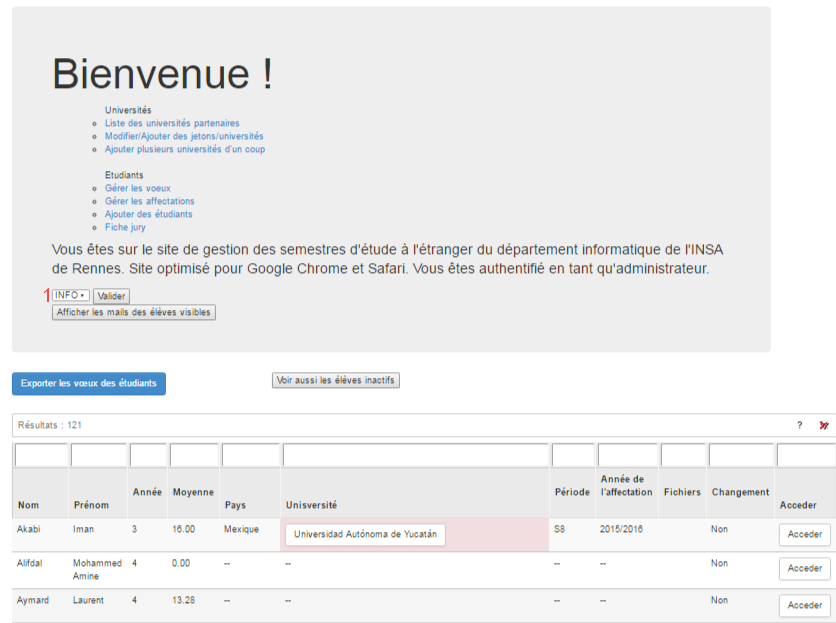
\includegraphics[width=16cm,height=10cm]{Images/Super_Admin/menu_acceuil_super_admin}
  	\caption{Accueil}
  	\label{asa}
  \end{figure}
  
    \subsection{Liste des universités partenaires}
    \begin{figure}[H]
    	\centering
    	
    	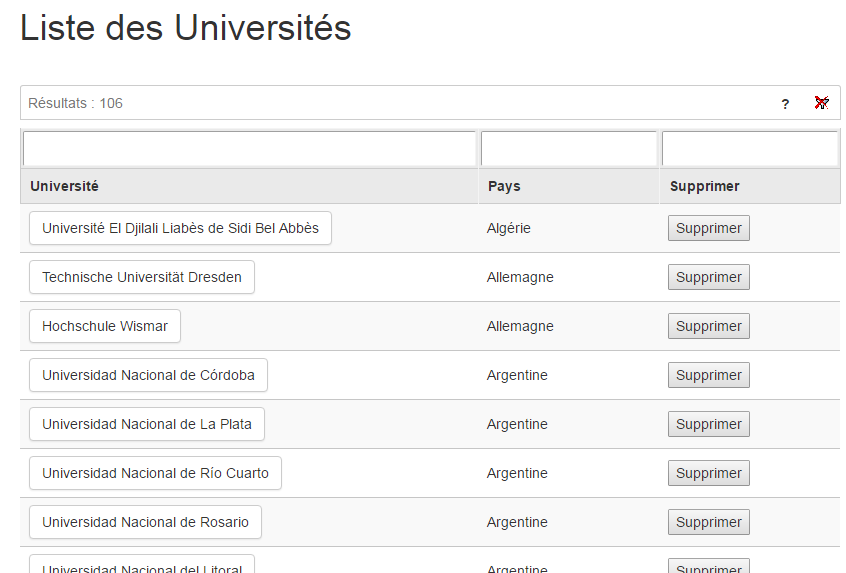
\includegraphics[width=16cm,height=12cm]{Images/Super_Admin/liste_univ_super_admin}
    	\caption{Liste des universités partenaires}
    	\label{lusa}
    \end{figure}
 
  \subsection{Ajout d'élèves ou d'administrateurs}
  \begin{figure}[H]
  	\centering
  	
  	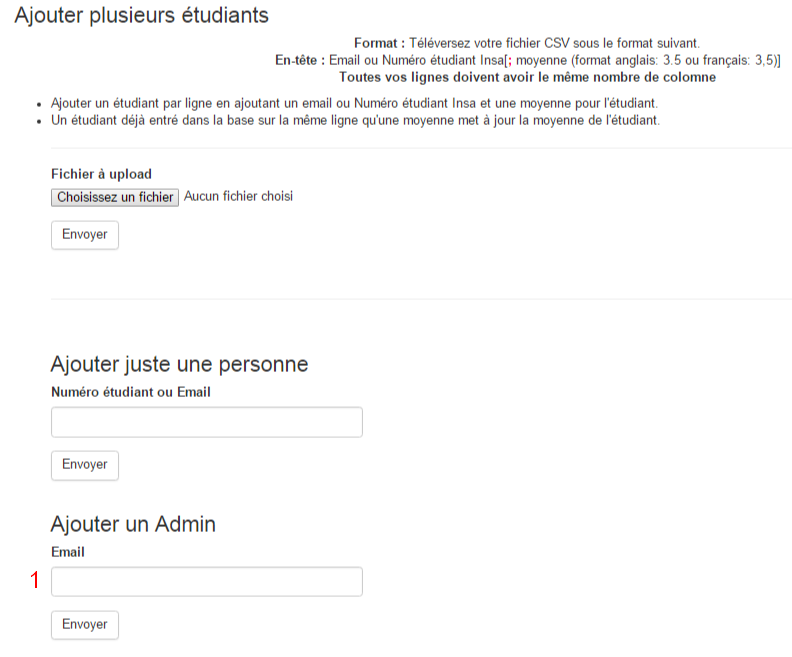
\includegraphics[width=16cm,height=12cm]{Images/Super_Admin/ajout_gens_super_admin}
  	\caption{Ajout d'élèves ou d'administrateurs}
  	\label{agsa}
  \end{figure}
    